\chapter{Metodologia}
\label{chap:metodologia}

Abans de començar a escriure cap línia de codi cal determinar quina és la metodologia que s'utilitzarà durant el projecte. 

Així en aquest s'ha utilitzat el model incremental o iteratiu. A més a més s'ha complementat amb la utilització de Test Driven Development per poder controlar de forma automatitzada el correcte funcionament de l'aplicació.

En els següents apartats es descriu amb més detalles les característiques d'aquestes dos metodologies.  


\section{Model Incremental o Iteratiu}

Per a la realització de tot el software relacionat amb el projecte s’ha utilitzat un model de procés del software incremental Aquest model aplica seqüències lineals de forma esglaonada a mesura que avança el temps. Cada seqüència lineal produeix un "increment" del software, i al utilitzar aquest model el primer increment sol ser un producte essencial, que no compleix ni els requisits bàsics.

\begin{figure}[htbp]
\centering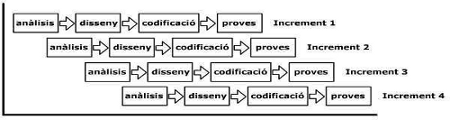
\includegraphics{img/model-incremental.png}
\caption{Cicle de desenvolupament del model incremental.}
\label{fig:mii}
\end{figure} 


Aleshores s’utilitza aquest producte per mostrar-lo al client i crear un pla pel següent increment. En cada increment el software ha de ser verificat i testat, per tal de evitar acumular errors al passar al següent increment. És un model molt útil quan volem anar entregant fases incompletes del sistema per tal que els client les puguin anar provant, i així, inclús podem afinar més en l’anàlisi dels requisits.

A la figura \ref{fig:mii} es pot veure un diagrama del cicle de desenvolupament basat en Test Driven Development.

Els avantatges d’utilitzar aquest model són:

\begin{itemize}
\item{Té en compte l’evolució del software.}
\item{Els primers increments permeten descobrir nous requeriments per a pròxims increments.}
\item{El client aviat rep versions operatives (encara que incompletes) del producte, i en conseqüència s’involucra més en el procés.}
\item{Funciona bé quan l’equip de programadors es reduït.}
\end{itemize}

Els inconvenients d’utilitzar aquest model són:

\begin{itemize}
\item{Problemes per determinar les funcionalitats a desenvolupar a cada increment.}
\end{itemize}

\section{Test Driven Development}
\label{sec:tdd}

Test Driven Development o desenvolupament de software bastat en Testos es una metodologia de desenvolupament de software centrada en els jocs de proves. Un joc de prova és una porció de codi que s'utilitza per comprovar de forma automàtica que el que es vol implementar funciona de forma correcta. Aquesta metodologia utilitza el següent cicle de desenvolupament: 

\begin{figure}[htbp]
\centering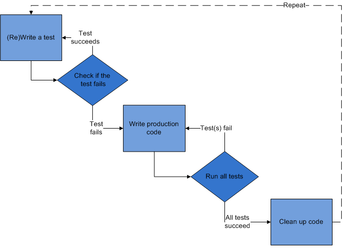
\includegraphics{img/test-driven-development.png}
\caption{Representació del cicle de desenvolupament basat amb TDD}
\label{fig:tdd}
\end{figure} 

\begin{enumerate}
    \item{Escriure un joc de prova.}
    \item{Executar tots els jocs de prova per comprovar que el nou test falla.}
    \item{Escriure el codi necessari per a que el joc de prova sigui favorable.}
    \item{Executar tots els jocs de provar per comprovar que tots els test són satisfactoris.}
    \item{Reestructurar el codi}
\end{enumerate}

A la figura \ref{fig:tdd} es pot veure un diagrama del cicle de desenvolupament basat en Test Driven Development.

Els passos descrits anteriorment es duen a terme per a cada nova funcionalitat que es vol implementar. Aquesta metodologia té l'objectiu d'implementar petites funcionalitats que puguin ser provades de forma independent per un joc de prova, per tal de desprès ajuntar-les amb el conjunt de l'aplicació. 

El Test Driven Development té les següents ventatges: 

\begin{enumerate}
    \item{Solidesa davant les fallades.}
    \item{Claredat dels requisits a implementar.}
    \item{Millora de la productivitat.}
\end{enumerate}

i els següents inconvenients: 

\begin{enumerate}
    \item{Difícil d'implementar en alguns casos: Interfícies de client,bases de dades, programes dependents de la xarxa }
    \item{Dependència de que els testos estiguin ben escrits. }
    
\end{enumerate}

